In this project, we address the 4 aforementioned challenges by designing an automatic and comprehensive test suite for synthesized scenes,
which provides ways for evaluating the authenticity of the rendering methods used in MSF-ADV\cite{msf-adv}.

\subsection{Overview}

To address the challenges in Section 5.2, our test suite has the following designs;

\textbf{Different driving backgrounds, 3D obstacle properties, and their interaction}. 
To address \textbf{C1}, through our preliminary experiments, we choose driving backgrounds with different degrees of crowdedness, 
The 3D obstacle with various colors, shapes, and textures, and the relative position between the background and the obstacle.
Fig. \ref{fig:test-pipe} is the overview of the automated test suite pipeline for the synthesized scenes.

For road backgrounds, 5 different driving scenarios are chosen according to the number of cars, the light condition, the shape of the road, and the emptiness of the road.
As we can notice, some background has more than 13 cars while for others there are only 2~5 cars.
The number of cars will influence the performance of the object detection neural network as it's easier to have occlusion between the obstacle with the cars in the background when there are more cars.
The result of the neural network will be quite sensitive to the position of the obstacle when the road is more crowded.
These 5 backgrounds are with different light conditions also. 
For some backgrounds, the shadow of the trees takes up half part of the road while in other backgrounds there is less shadow on the road and even now shadows.
The shadow area will affect the object detection accuracy in a way that obstacles put in the shadow are harder to be detected, 
especially when the color of the obstacle is quite dark.

For 3D obstacle properties, we first choose different shapes of objects of the same type.
Considering that the chair is quite common and easy to obtain in real life, 
we choose the chair as our target benign obstacle and also use 3 different shapes of the chair for generality.
We also change the color and the facing angle of the chair.
The original color is wood brown, however, this is easy not to be detected when it's under shadow or close to the soil.
Therefore we also choose bright colors, i.e., blue and pink for the chair.
Also, we rotate the chair for random angles as the angles in which the chair is put will also affect the detection performance.
A chair with a full view will be detected easily while a chair with only a side view is harder to be detected and recognized as the chair.

For the interaction between the obstacle and the background, we adjust the position of the chair on both the x-axis and y-axis.
For a chair that is close to the camera, it's easier to be detected while for a chair that is far from the camera, it's the opposite case.
We implement the distance between the chair and the camera by adjusting its position on the x-axis.
The position of the chair will affect the occlusion. 
For example, if the chair is on the left side of the road and there happens to be a car here. 
The chair may block the car and prevent it to be detected.
However, if the chair is on the right side, there won't be occlusion then.

The attacker can easily simulate this by choosing an object with different shapes and colors and putting it on the road.

\textbf{Adjust the size of the object along with its position.}
To address \textbf{C2}, we adopt camera imaging theory to adjust the height of the object so that it's standing on the road.
For example, if the obstacle is far from the camera, simply cropping the obstacle image and integrating it with a farther position on the x-axis won't help.
It's likely to hit the road as the size of the obstacle should also shrink along with the increase of the distance to the camera.
In the same way, if the obstacle is close to the camera, simply moving it closer on the x-axis will likely cause the object to float in the air.
The size of the object should also increase when it's closer to the camera.
We do experiments on our backgrounds and take the following equation to model the relationship between the obstacle size and the distance between it and the camera.
\begin{equation}
	z = -1.73 + r/2
\end{equation}
Here \(z\) represents the distance between the obstacle and the camera in the unit of meters. \(r\) represents the scaling factor of the size of the obstacle.
Moving the obstacle away or closer to the camera with the corresponding scaling factor in the equation ensures 
that the obstacle is standing on the ground without floating or hitting the ground.

On the other hand, we also consider the light condition to comply with the driving background.
When there is a shadow in the background which is caused by the sunlight from a certain direction, 
an obstacle putting on the road should also have a similar shadow to ensure physical consistency.
To produce a similar light condition, 
we consider the direction and intensity of the light when we're using the camera rendering function to get the 2D image.
Also, we start with normal obstacles which can be obtained from
life easily, e.g., a common chair.
This is a fair assumption as getting the original obstacle shouldn't be difficult for the attacker.

\textbf{Detection rate and Confidence rate}
To address \textbf{C3}, we parse the output of object detection neural networks, i.e., detected bounding box, object label, and confidence scores.
Then we introduce two metrics, i.e., detection rate and confidence rate to measure the performance of the neural networks.
Specifically, Fig. \ref{fig:algo} shows the overview of the algorithm to get the total confidence scores and the correctly detected objects.
Here we choose YOLOv3 as our target neural network as it's used in Autoware.AI\cite{autoware} for object detection. 
The output of YOLOv3 includes the bounding box, label, and confidence score.
The bounding box is used to describe the position of the detected object. 
The most important part of object detection is detecting the obstacle in the right place.
Here we use the Intersection over Union(IoU) to describe the extent of overlap of two objects.
Fig. \ref{fig:iou} shows the equation to calculate IoU.
We divide the area of overlap of two objects, i.e., the ground truth bounding box and the detected bounding box, with the area of the union of two objects.
If the calculated IoU is close to 1, it means the detected bounding box almost overlaps with the ground truth and the detection position for the obstacle is correct.
We set a threshold $\alpha$ to compare with the calculated IoU to decide if the detection position is correct.

Then the label of the obstacle is chosen and compared with the ground truth label.
If they match, it means that the detected obstacle is correctly classified.
And we think this obstacle is detected correctly. 
Therefore we record the confidence score of this detection result and count this as a correctly detected object.

In the end, we use the equation in Fig. \ref{fig:detection} and Fig. \ref{fig:conf} to calculate the detection rate and confidence rate.
The detection rate is used to measure the percentage of correctly detected objects 
and the confidence rate is used to measure the average confidence scores per object.
By comparing these two metrics in synthesized scenes with different settings, 
we can evaluate the performance of the neural network and therefore the authenticity of these scenes.

\textbf{Automated pipeline for test suites} 
To address \textbf{C4}, we need to design automated pipelines for the whole testing process to improve efficiency.
In Fig. \ref{fig:test-pipe}, we first randomly choose one kind of chair as our target obstacle.
Then we randomly choose the color between wood brown, blue and pink.
The colored chair will be rotated at a random angle in [0\textdegree, 180\textdegree].
Meanwhile, a road background will be picked randomly to serve as the driving scenario.
We also shift the position of the chair on both the x-axis and the y-axis.
The shifting range in the x-axis is set to be in [4m, 8.5m] and the shifting range in the y-axis is set to be in [-8m, 8m].
While we're shifting the obstacle, we also scale the size of the object according to the camera imaging equation to ensure physical consistency.
Then we render this obstacle with a certain background to get the 2D images.
This camera image is sent to the object detection neural network to get the detection rate and confidence rate of the final outputs.
These are used to measure the authenticity of the benign synthesized image.

In Fig. \ref{fig:test-att}, we generate the adversarial obstacle using MSF-ADV\cite{msf-adv}.
Then we render the adversarial object with the camera rendering function and integrate it with the background. 
The generated 2D image is fed into the camera object detection neural network to get the detection rate and confidence rate of the adversarial synthesized scene.
This is to measure the effectiveness of generated adversarial obstacles in the road background.

%-----------


\begin{figure}
	\centering
	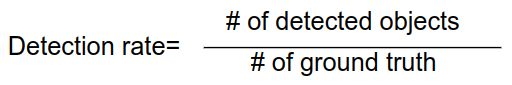
\includegraphics[width=0.7\linewidth]{figure/detection.png}
	\caption{Detection rate.}
	\label{fig:detection}
\end{figure}

\begin{figure}
	\centering
	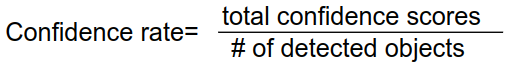
\includegraphics[width=0.7\linewidth]{figure/confidence.png}
	\caption{Confidence rate.}
	\label{fig:conf}
\end{figure}
%
\begin{figure}
	\centering
	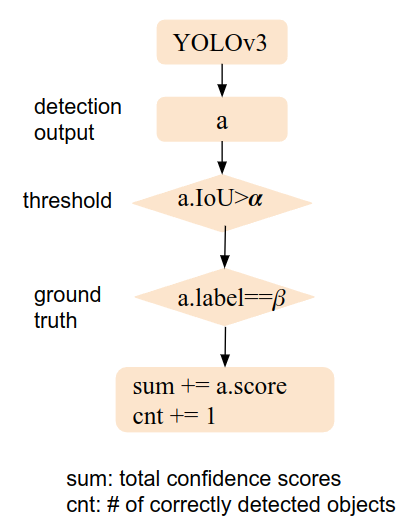
\includegraphics[width=0.5\linewidth]{figure/algorithm.png}
	\caption{Algorithm for calculating confidence scores and detected objects.}
	\label{fig:algo}
\end{figure}


\begin{figure*}
	\centering
	\begin{subfigure}{0.5\textwidth}
		\centering
		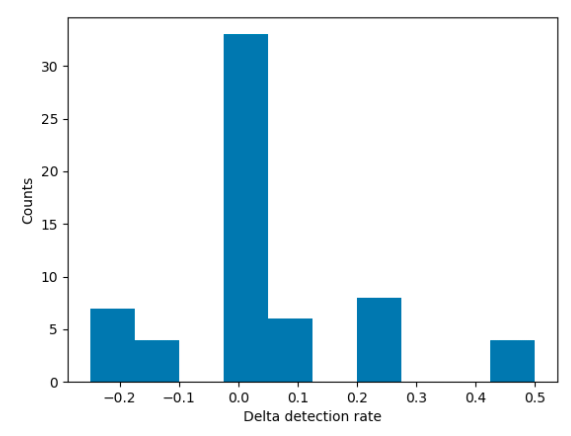
\includegraphics[width=0.7\linewidth]{figure/detection-de.png}
		\caption{Delta detection rate}
		\label{fig:det-d}
	\end{subfigure}%
	\begin{subfigure}{0.5\textwidth}
		\centering
		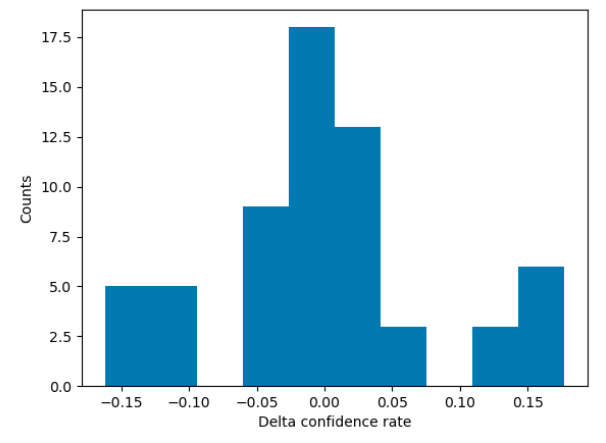
\includegraphics[width=0.7\linewidth]{figure/conf-de.png}
		\caption{Delta confidence rate}
		\label{fig:conf-d}
	\end{subfigure}
	\caption{Delta detection rate and confidence rate between benign objects and adversarial ones.}
	\label{fig:delta}
\end{figure*}

%\begin{figure*}
%	\centering
%	\begin{subfigure}{0.5\textwidth}
%		\centering
%		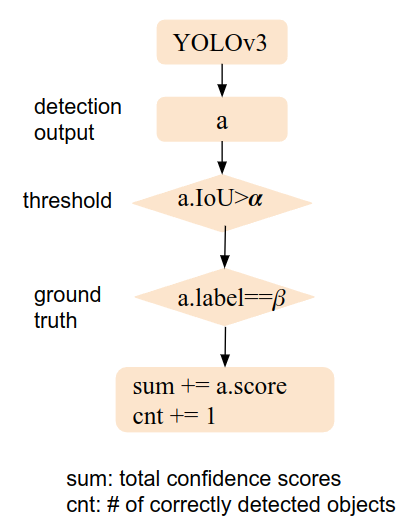
\includegraphics[width=0.7\linewidth]{figure/algorithm.png}
%		\caption{Algorithm for calculating confidence scores and detected objects.}
%		\label{fig:algo}
%	\end{subfigure}%
%	\begin{subfigure}{0.5\textwidth}
%		\centering
%		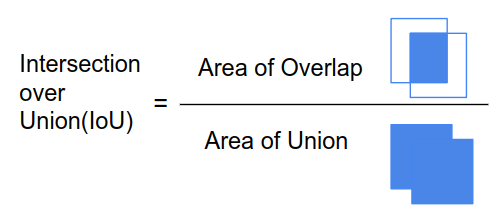
\includegraphics[width=0.7\linewidth]{figure/iou.png}
%		\caption{Intersection over Union(IoU)}
%		\label{fig:iou}
%	\end{subfigure}
%	\caption{Water treatment plant architecture and Attack Model}
%	\label{fig:swat}
%\end{figure*}

%-----------

%Adversarial 3D objects usually have noisy surfaces to mislead the detection networks.
%Thus, surface denoising is needed in the pre-processing unit.
%Directly applying the object reconstruction network like IF-Defense\cite{if-defense} will result in high computational overhead and low performance.
%Thus, we design a lightweight segmentation algorithm to first crop the potential areas containing obstacles based on laser imaging theory,
%and then apply IF-Defense\cite{if-defense} to recover the surface of the 3D object. 
%
%\subsection{Characteristics of adversarial 3D objects}
%
%Adversarial 3D objects are generated by adding, removing, and modifying the 3D points.
%These perturbations, however, will always lead to a rough object surface, violating the geometrical features in Figure~\ref{fig:noisy}(b).
%When the distance between the vehicle and the adversarial obstacle is larger than the brake distance,
%it is easy for the vehicle to mistake this glitchy surface as noise and ignore the overall shape of the obstacle.
%In this case, it fails to detect the obstacle and crashes into it.
%Therefore, it's important to smooth the noise on the surface and let the out-of-bound points lie on the surface.
%
%\subsection{Recovering methods}
%
%For 3D point clouds, there are broadly two types of methods to recover the distorted surface of 3D adversarial objects.
%One is traditional filtering based methods such as VG\cite{VG}, L0\cite{L0}, MLS\cite{mls}. They perform well in removing overall noise in the 3D perception but fail to recover the broken surfaces.
%The other is deep neural network based object reconstruction methods such as DUP-Net\cite{dupnet} and IF-Defense\cite{if-defense}.
%They aim to recover the broken surface and local part removal attack.
%
%However, they are only evaluated on a single 3D object instead of the outdoor scene perceived by autonomous cars.
%It is difficult to apply them directly in AV perception because 1) it will induce large unnecessary computation overhead as the whole road condition is fed as the input, 
%and 2) the object reconstruction methods are mostly trained on single object datasets instead of real AV outdoor datasets.
%
%Therefore, in this defense, we first design our own lightweight segmentation algorithm in real AV perception, 
%and then apply the latest object reconstruction method - IF-Defense\cite{if-defense}, to remove the noise on the surface.
%
%In the following parts, we first introduce our lightweight segmentation algorithm and then introduce the segmentation-based IF-Defense\cite{if-defense}.
%
%% For 2D images, smoothing can be done with varies filtering methods such as mean filtering\cite{mean-filter} and median filtering\cite{median-filter} 
%% and they work quite well.
%
%%% ADD figure 
%
%%\begin{figure}
%%	\centering
%%	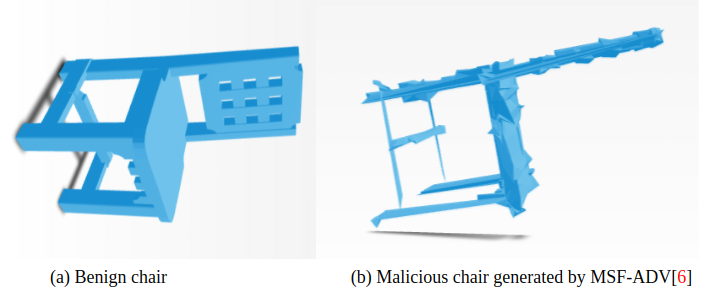
\includegraphics[width=1\linewidth]{figure/benign&ma.png}
%%	\caption{Benign chair and the malicious version}
%%	\label{fig:noisy}
%%\end{figure}
%
%% \begin{figure*}
%% 	\centering
%% 	\begin{subfigure}{0.5\textwidth}
%% 		\centering
%% 		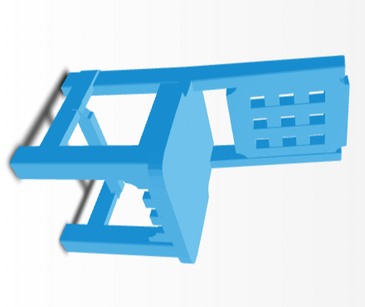
\includegraphics[width=0.6\linewidth]{figure/benign.png}
%% 		\caption{Benign chair}
%% 		\label{fig:benign}
%% 	\end{subfigure}%
%% 	\begin{subfigure}{0.5\textwidth}
%% 		\centering
%% 		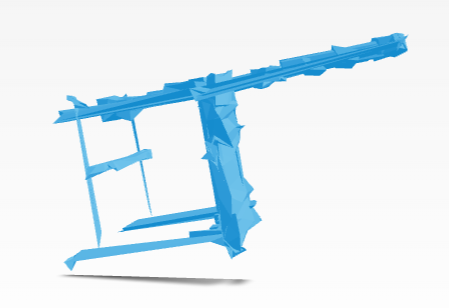
\includegraphics[width=0.7\linewidth]{figure/malicious.png}
%% 		\caption{Malicious chair generated by MSF-ADV\cite{msf-adv}}
%% 		\label{fig:noisy}
%% 	\end{subfigure}
%% 	\caption{Water treatment plant architecture and Attack Model}
%% 	\label{fig:benign&noisy}
%% \end{figure*}
%
%\subsection{Lightweight segmentation algorithm}
%
%Figure~\ref{fig:lidar} is an example of projected LiDAR perception of a traffic cone in the middle of the road. 
%These wave-like curves are the result of laser scanning in an open area.
%An obstacle will prevent the laser from scanning the area behind it and thus a blank area is formed behind the obstacle.
%We can therefore use these white areas to segment the potential areas containing the obstacle.
%After that, applying IF-Defense\cite{if-defense} only in these segmented areas will reduce the computation workload.
%
%To segment these areas, we first project the 3D object point cloud with a front view like Figure~\ref{fig:lidar} to get the image of 2D points.
%Then we divide the 2D projection into multiple cells illustrated in Figure~\ref{fig:seg}(a).
%% How to decide a?
%The cell is a square with the edge length \emph{a} to help us calculate the points' distribution. % Add figure
%We then calculate the total amount of points in the cell and store it, like in Figure~\ref{fig:seg}(b).
%Algorithm~\ref{alg:segment} shows how we get the potential segmentation areas.
%
%% We slide the cell with step \emph{d} horizontallly and vertically from one vertex to another until it walks through every 3D points.
%
%From the observation in Figure~\ref{fig:lidar}, obstacles usually have higher point density followed by a blank shadow-like area. 
%Therefore, our goal is to find dense cells which are also accompanied by a series of sparse cells.
%First, in Line 7, we sort the array of the number of points in each cell, choose the top \emph{c}\% dense cell numbers as our obstacle set \emph{A} in Line 8, and choose the least \emph{d}\% dense cell as our blank area set \emph{B} in Line 9.
%In Line 10, we select one cell \emph{i} from \emph{A}, calculate the Manhattan distance between the \emph{i} and each cell in set \emph{B} according to Eq.~\ref{eq:Manhattan}.
%
%In Eq.~\ref{eq:Manhattan}, $A(i)_x$ represents the $x$ coordinate of $i_{th}$ cell in $A$, i.e., the obstacle set.
% $A(i)_y$ represents the $y$ coordinate of $i_{th}$ cell in $A$.
% $B(i)_x$ represents the $x$ coordinate of $i_{th}$ cell in $B$, i.e., the blank area set.
% $B(i)_y$ represents the $y$ coordinate of $i_{th}$ cell in $B$.
% And the Manhattan distance $d_{ij}$ is the sum of the absolute differences of the coordinates of two points.
%We choose this metric because it's fast to calculate and also represents how far two points are from each other. 
%
%Then in Line 15, we sort the array of Manhattan distance $D$ in ascending order.
%We further calculate the Manhattan distance among the top \emph{k}\% cells in $D$ in Line 18, to measure the distances among blank area cells. 
%In Line 19, we add all the Manhattan distances in $D$ and compare it with a threshold.
%If the sum is lower than a threshold \emph{h}, we think these cells are close to each other and might be shadows of the obstacle.
%Then we choose the highest and lowest \emph{x} and \emph{y} coordinates of the points and serve this as the segmentation boundary.
%Algorithm~\ref{alg:segment} ends when all the obstacles in set A are iterated.
%We note that parameters in the algorithm like $c$, $d$, $k$, and $threshold$ have to be decided by experiment and profiling.
%
%\begin{equation}
%    \label{eq:Manhattan}
%    d_{ij} = |A(i)_x - B(j)_x| + |A(i)_y - B(j)_y|
%\end{equation}
%
%\begin{algorithm}[h]
%    \caption{Object segmentation algorithm}\label{alg:segment}
%    \begin{algorithmic}[1]
%    \State $num\_Array$: array of the number of points in each cell
%    \State $A$: obstacle sets
%    \State $B$: blank area sets
%    \State $D$: Manhattan distance array
%    \State $sum\_Dis$: Sum of difference in Manhattan distance
%    \State $bound\_Dict$: Boundaries of each segmentation
%    \State Sort $num_Array$ in descending order
%    \State $A$ $\gets$ Top c\% elements in $num_Array$
%    \State $B$ $\gets$ Least d\% elements in $num_Array$
%    % \State $p\_Array$: final pattern array
%    % \State $p\_Dict$: dictionary of detected pattern
%    % \State $idx$: the number of elements to match
%    % \State $idx \gets 2$ 
%    % \State $p \gets arrayofPac[0:1]$
%    \While{$A$ is not fully checked}
%        \While{$B$ is not fully checked}
%            \State $d_{ij}$ = |$A(i)_x$ - $B(j)_x$| + |$A(i)_y$ - $B(j)_y$|
%            \State add $d_{ij}$ into $D$
%        \EndWhile
%        \State Sort $D$ in ascending order
%        \State $D$ $\gets$ Top $k$\% $D$
%
%        \While{$D$ is not fully checked}
%            \State $diff$ = |$D(i)_x$ - $D(i+1)_x$| + |$D(i)_y$ - $D(i+1)_y$| 
%            \State $sum\_Dis$ += $diff$
%        \EndWhile
%        \If{$sum\_Dis$ < $threshold$}
%            \State $bound\_Dict[i]$ $\gets$ smallest $x$ coordinate in $D$
%            \State $bound\_Dict[i]$ $\gets$ largest $x$ coordinate in $D$
%            \State $bound\_Dict[i]$ $\gets$ smallest $y$ coordinate in $D$
%            \State $bound\_Dict[i]$ $\gets$ largest $y$ coordinate in $D$
%        \EndIf
%    \EndWhile
%    \State return $bound\_Dict$
%    \end{algorithmic}
%    \end{algorithm}
%
%\begin{figure}
%	\centering
%	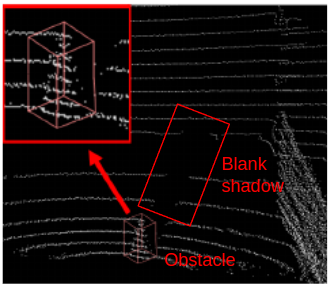
\includegraphics[width=0.5\linewidth]{figure/lidar.png}
%	\caption{LiDAR perception. Modified from Figure 10 in \cite{msf-adv}}
%	\label{fig:lidar}
%\end{figure}
%
%\begin{figure*}
%	\centering
%	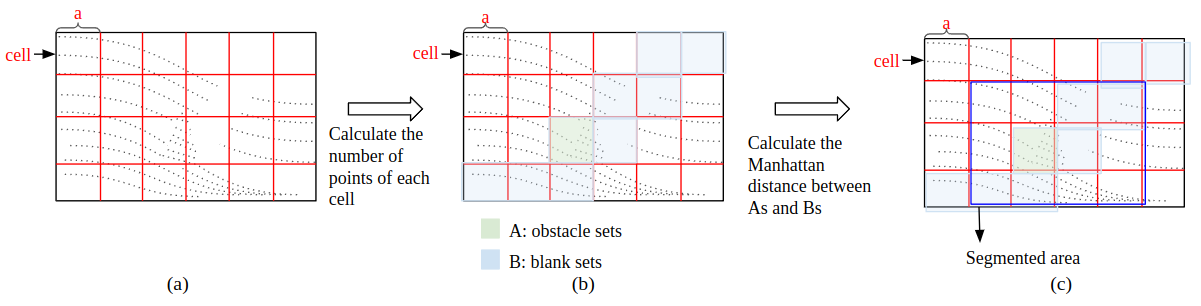
\includegraphics[width=1\linewidth]{figure/segmentation.png}
%	\caption{Segmentation algorithm}
%	\label{fig:seg}
%\end{figure*}
%
%
%
%\subsection{Segmentation-based IF-defense} 
%IF-defense\cite{if-defense} is a framework to recover the corrupted surface of the point cloud based on the implicit function\cite{implicit}.
%It aims to optimize the shape of 3D objects to follow the geometry property and realize the uniform distribution of 3D points.
%It uses geometry-aware and distribution-aware loss functions to encourage the optimized points to lie on the surface as well as distribute more evenly.
%IF-defense\cite{if-defense} is implemented with ONet\cite{ONet} and ConvONet\cite{ConvONet} network.
%However, the dataset that IF-defense\cite{if-defense} uses is ShapeNet\cite{shapenet}, which is a set of single clean 3D objects.
%It hasn't been tested on AV scenarios such as the KITTI\cite{kitti} dataset. 
%
%One big challenge of applying it on point clouds in AV outdoor perception is that there are multiple objects existing in the scene, like roads, buildings, vehicles, and pedestrians.
%Since we aim at removing the obstacle noises fed into the object detection network, recovering the whole point cloud including the road is a waste of resources.
%Also, it may not perform well in AV outdoor perception due to the different training dataset.
%
%Thus, we plan to first use the lightweight segmentation algorithm to get the potential recovery areas.
%Then we apply the IF-defense\cite{if-defense} to recover the selected areas.
%At last, we replace the originally selected point clouds with the recovered point clouds and feed the combined output into the pre-processing unit in the AV perception module. 
%In this way, we hope to recover the LiDAR detection output before sending it to the sensor fusion part.
